\chapter{Project Risk Assessment \& Management}

\section{Project Risk Assessment}   \label{sec:risk_assessment}
Based on a group discussion, seven key risks were identified regarding the organisation and management of the project. These included: cloud service failure, encountering a bottleneck in the design process, miscommunication between team members, external/internal advice delay, poor time estimation, interpersonal conflict and absence of team members. A likelihood score and a severity score were assigned to each risk based on its possible influence on the project. The resulting risk map can be seen in \autoref{fig:risk_matrix}.

\begin{figure}[h]
    \centering
    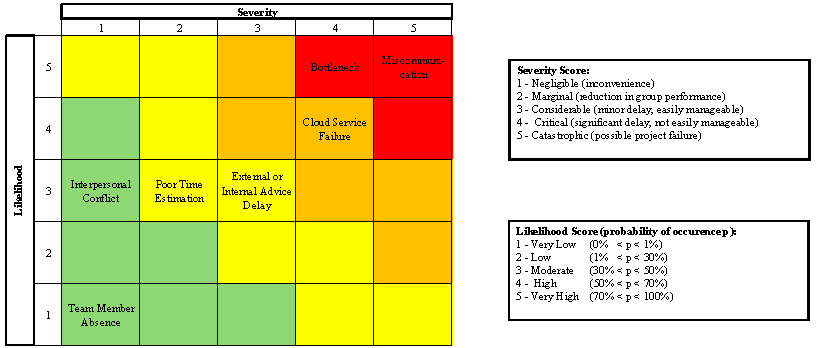
\includegraphics[width=1\linewidth]{figures/risk_matrix-4.pdf}
    \caption{Project Risk Map}
    \label{fig:risk_matrix}
\end{figure}

Based on the risk analysis, three crucial project risks were identified. Miscommunication between team members was estimated as very likely to occur, with a possibly catastrophic impact if not acted upon immediately. A design bottleneck (scenario in which a delay in one task disrupts the flow of multiple other tasks or parts of the project) was also identified as a risk of potentially catastrophic results, with a high possibility of occurrence (especially if combined with miscommunication). Additionally, cloud service failure was chosen as a key risk based on the experience of previous year's teams. Therefore, it was decided that risk management plans shall be drafted for each of the aforementioned scenarios.

\section{Risk Management Plans} \label{sec:risk_management}
A risk management plan shall incorporate both preventative measures and contingency plans to reduce both the likelihood and impact severity for each scenario. In this Section, such plans are developed for each of the crucial project risks identified in \autoref{sec:risk_assessment}.

\subsection{Miscommunication}
Miscommunication between team members is, by far, the most severe and common risk for an engineering project. If not addressed and identified soon enough, it can have catastrophic consequences. Examples of miscommunication scenarios include:
\begin{itemize}
    \item A team member performing their tasks with no communication with the rest of the team, then discovering that their results do not match the outputs of the rest of the group.
    \item Several subteams developing parts of the aircraft independently, then realizing that their outputs are not compatible.
    \item A team member missing a session without prior notice, disrupting the flow and schedule of the project.
\end{itemize}

\subsection{Bottleneck}

\subsection{Cloud Service Failure}
